\documentclass[12pt,fleqn]{article}\usepackage{../../common}
\begin{document}
Frekanslar, Uygulamalar

Adim Olcmek, Pedometre

\begin{minted}[fontsize=\footnotesize]{python}
import pandas as pd
dfacc = pd.read_csv('acc.txt',header=None,sep='\s+')
print dfacc.head()
\end{minted}

\begin{verbatim}
               0         1         2         3
0  1493818386218 -0.147100  6.972528  6.707748
1  1493818386422 -0.215746  7.001948  6.854848
2  1493818386610 -0.304006  7.041174  6.697942
3  1493818386812 -0.304006  7.050981  6.884268
4  1493818387008 -0.225553  7.011754  6.943108
\end{verbatim}

\begin{minted}[fontsize=\footnotesize]{python}
steps = np.sqrt(np.sum(dfacc[[1,2,3]]**2, axis=1))-10.0
steps[:200].plot()
plt.savefig('tser_freq_01.png')
\end{minted}

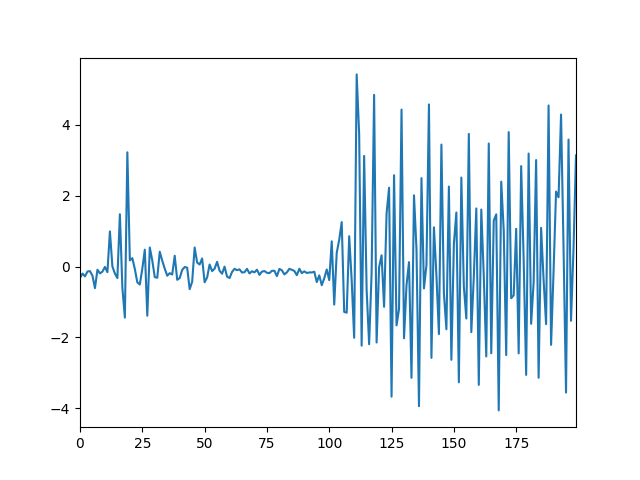
\includegraphics[height=6cm]{tser_freq_01.png}

\begin{minted}[fontsize=\footnotesize]{python}
fs = 20
fou = np.fft.fft(steps, fs)
hmag=np.real(fou); ah=hmag/len(steps);
f=plt.figure()
plt.stem(ah)
plt.savefig('tser_freq_02.png')
\end{minted}

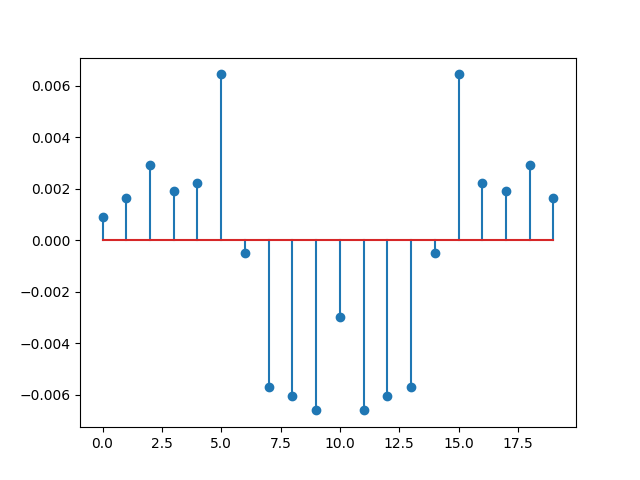
\includegraphics[height=6cm]{tser_freq_02.png}

Radyo Dalgalari

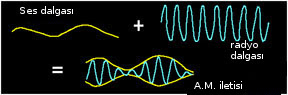
\includegraphics[width=20em]{AM_waves.jpg}

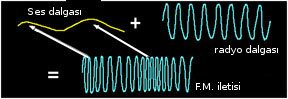
\includegraphics[width=20em]{FM_waves.jpg}

\inputminted[fontsize=\footnotesize]{python}{FMDemodulator.py}

[devam edecek]

Kaynaklar

[1] {\em The Basic Facts About Radio Signals}, \url{https://www.windows2universe.org/spaceweather/wave_modulation.html}

[2] \url{https://www.dropbox.com/s/lpwz2iby0nhh8p7/fm1.dat?dl=1}

[3] \url{https://www.dropbox.com/s/70adji6wyst0qbi/fm2.dat?dl=1}

[4] Scher, {\em How to capture raw IQ data from a RTL-SDR dongle and FM demodulate with MATLAB},\url{http://www.aaronscher.com/wireless_com_SDR/RTL_SDR_AM_spectrum_demod.html}

[5] {\em EE123: Digital Signal Processing}, \url{http://inst.eecs.berkeley.edu/~ee123/sp14/}

[6] Fund, {\em Capture and decode FM radio}, \url{https://witestlab.poly.edu/blog/capture-and-decode-fm-radio/}

[7] Fund, {\em Lab 1: Working with IQ data in Python}, \url{http://witestlab.poly.edu/~ffund/el9043/labs/lab1.html}

[8] Barton, {\em Nest Interview}, \url{https://github.com/sbarton272/Pedometer}

\end{document}




















